\documentclass[12pt]{article}
\usepackage{mathtext}
\usepackage{amsmath}
\usepackage[T2A]{fontenc}
\usepackage[utf8]{inputenc}
\usepackage[russian]{babel}
\usepackage[left=1.5cm, right=1.5cm, top=2cm, bottom=2cm, bindingoffset=0cm]{geometry}
\usepackage{listings}
\usepackage{fancyhdr}
\usepackage{pgfplots}
\pgfplotsset{compat=1.9}

\begin{document}
    \begin{center}
        \textbf{Московский авиационный институт} \\
        \textbf{(Национальный исследовательский университет)}
    \end{center} 
    ~\\
    ~\\
    Институт: «Информационные технологии и прикладная математика» \\
    Кафедра: 804 «Теория вероятностей и компьютерное моделирование» \\
    Дисциплина: «Математическое моделирование»  
    ~\\
    ~\\
    ~\\
    \begin{center}
        Лабораторная работа №2 \\
        Тема: Метод Линдштедта
    \end{center}
    ~\\
    ~\\
    ~\\
    ~\\
    ~\\
    ~\\
    ~\\
    ~\\
    ~\\
    \begin{flushright}
        Студент: ~~~~~~~Хахин Максим~~~~~~~~~~~\\
        Группа: ~~~~~~~~~~~~80-403~~~~~~~~~~~~~~~~~~~\\
        Преподаватель:~~~~~~~ Майоров А. Ю.\\
        Дата: ~~~~~~~~~~~~~~~~~~~~~~~~~~~~~~~~~~~~~~~~~~~\\
        Оценка:~~~~~~~~~~~~~~~~~~~~~~~~~~~~~~~~~~~~~~~~~\\
    \end{flushright}
    ~\\
    ~\\
    ~\\
    ~\\
    ~\\
    ~\\
    ~\\
    ~\\
    ~\\
    ~\\
    ~\\
    ~\\
    ~\\
    ~\\
    ~\\
    \begin{center}
        Москва, 2021
    \end{center}
    \pagestyle{empty}
    \newpage

    \pagestyle{fancy} 
        \fancyhead{}
        \fancyhead[L]{Хахин Максим}
        \fancyhead[R]{М8О-403Б-18} 
    \fancyfoot{} 

    Колебания механической системы описываются уравнением:
    \begin{eqnarray}
        \ddot{x} + x+ \frac{x^3}{\sqrt{{ (x^2 + 1)^3 }}} = 0.
    \end{eqnarray}
    \begin{itemize}
        \item[a)]
        Разложим функцию $f(x)= x+ \frac{x^3}{\sqrt{{ (x^2 + 1)^3 }}}$ в ряд Тейлора в окрксности точки равновесия $x^*=0$:
        $$f(x)= f(x^*)+f'(x^*)(x-x^*)+\frac{f''(x^*)}{2}(x-x^*)^2+\frac{f'''(x^*)}{6}(x-x^*)^3+О((x-x^*)^4$$
        \begin{itemize}
            \item $f'(x)=\frac{3x^2}{(1+x^2)^{3/2}}-\frac{3x^4}{(1+x^2)^{5/2}}+1;\:f'(0)=1$
            \item $f''(x)=\frac{15x^5}{(1+x^2)^{7/2}}-\frac{21x^3}{(1+x^2)^{5/2}}+\frac{6x}{(1+x^2)^{3/2}};\:f''(0)=0$
            \item $f'''(x)=-\frac{105x^6}{(1+x^2)^{9/2}}+\frac{180x^3}{(1+x^2)^{7/2}}-\frac{81x}{(1+x^2)^{5/2}}+\frac{6}{(1+x^2)^{3/2}};\:f'''(0)=6$
        \end{itemize}
        \begin{eqnarray} f(x)=x-x^3+О(x^5)\Leftrightarrow \frac{x^2}{\sqrt{{ (1+x^2)^3 }}}+x=x+x^3.\end{eqnarray}
        Сделаем замены.
        \begin{enumerate}
            \item Подставим $x=\varepsilon y,\:\:\ddot x = \varepsilon \ddot y$ и запишем уравнение движеия:
            $$\varepsilon \ddot y+\varepsilon y+(\varepsilon y)^3=0$$
            \item $t=\omega \tau$
            $$\frac{d^2}{dt^2}=\omega^2\frac{d^2}{d\tau^2}$$
            \begin{eqnarray}\omega^2\varepsilon\frac{d^2y(\tau)}{d\tau^2}+\varepsilon y+(\varepsilon y)^3=0.\end{eqnarray}
        \end{enumerate}
        Сократив в (3) $\varepsilon$, становитя очевидно, что это уравнение вида:
        $$\omega^2y''+\omega_0y=\varepsilon f(y),$$
        откуда $\omega_0=1$.\\
        Зная, что $\omega=\omega_0+\varepsilon\omega_1+\varepsilon^2\omega_2+\varepsilon^3\omega_3$ запишем (3) в виде:
        \begin{eqnarray}
            (\omega_0+\varepsilon\omega_1+\varepsilon^2\omega_2+\varepsilon^3\omega_3)^2\frac{d^2y(\tau)}{d\tau^2}+y-\varepsilon^2y^3=0.
        \end{eqnarray}
        Теперь в (4) сделаем замену $y(\tau)=y_0(\tau)+\varepsilon y_1(\tau)+\varepsilon^2y_2(\tau)+\varepsilon^3y_3(\tau)$
        \begin{eqnarray}
            (\omega_0+\varepsilon\omega_1+\varepsilon^2\omega_2+\varepsilon^3\omega_3)^2\frac{d^2}{d\tau^2}(y_0(\tau)
            +\varepsilon y_1(\tau)+\varepsilon^2y_2(\tau)+\varepsilon^3y_3(\tau))+(y_0(\tau)+\varepsilon y_1(\tau)+
            \varepsilon^2y_2(\tau)+\varepsilon^3y_3(\tau))+\nonumber
            \\+\varepsilon^2(y_0(\tau)+\varepsilon y_1(\tau)+\varepsilon^2y_2(\tau)+\varepsilon^3y_3(\tau))^3=0.
        \end{eqnarray}
        \newpage
        Сгруппируем (5) по степеням $\varepsilon$, а затем применим разложение по малому:
        \begin{itemize}
            \item Решим Задачу коши для части уравнения без $\varepsilon$:
            \begin{equation*}
                \begin{cases}
                    \omega_0^2\ddot y_0(\tau)+y_0(\tau)=0 \\
                    y_0(0)=y_0\\
                    \dot y_0(0)=0
                \end{cases}
            \end{equation*}
            решением этой задачи имеет вид: $y_0(t)=A*cos(t)$.
            
            \item Решим Задачу коши для части уравнения c $\varepsilon^1$:
            \begin{equation*}
                \begin{cases}
                    2\omega_1\frac{d^2}{d\tau^2}A*cos(\tau) + \frac{d^2}{d\tau^2}y_1(\tau) + y_1(\tau)=0 \\
                    y_1(0)=0\\
                    \dot y_1(0)=0
                \end{cases}
            \end{equation*}
            решением этой задачи имеет вид: $y_1(\tau) = \omega_1A*sin(\tau)\tau$. Подставив $y_1(\tau)$ в исходное определим:
            $\omega_1=0$

            \item Решим Задачу коши для части уравнения c $\varepsilon^2$:
            \begin{equation*}
                \begin{cases}
                    \frac{d^2}{d\tau^2}y_2(\tau) + 2\omega_2A\frac{d^2}{d\tau^2}cos(\tau) + y_2(\tau) + A^3cos(\tau)^3 = 0 \\
                    y_2(0)=0\\
                    \dot y_2(0)=0
                \end{cases}
            \end{equation*}
            решением этой задачи имеет вид: $$y_2(\tau) = cos(\tau)\left(\frac{1}{4}A^3 - \omega_2A\right) - 
            \frac{3A}{8}\left(-\frac{A^2cos(\tau)^3}{3} + \left(A^2 - \frac{8\omega_2}{3}\right)cos(\tau) + 
            sin(\tau)\tau\left(A^2 - \frac{8\omega_2}{3}\right)\right).$$
            Занулим коэффициент при сикулярном члене $sin(\tau)\tau$ и вычислим $\omega_2$:
            $$A^2 - \frac{8\omega_2}{3}=0 \Rightarrow \omega_2=\frac{3A^2}{8}.$$
        \end{itemize}
        Таким образом, после всех подстановок получаем:
        \begin{eqnarray}
            y_0(\tau)=cos(\tau)A,\:\:y_1(\tau)=0,\:\:y_2(\tau)=-\frac{cos(\tau)A^3}{8} + \frac{cos(\tau)^3A^3}{8}
        \end{eqnarray}
        В таком случае получаем приблеженное решение вида:
        \begin{eqnarray}
            y(\tau)=cos(\tau)A-\frac{cos(\tau)A^3}{8} + \frac{cos(\tau)^3A^3}{8}.
        \end{eqnarray}
        Сделаем обратные замены $\tau=\omega_0t=t$ и $y(t)=y_0(\tau)+\varepsilon y_1(\tau)+\varepsilon^2y_2(\tau)$:
        \begin{eqnarray}
            y(t)=cos(t)A-\varepsilon^2\left(\frac{cos(t)A^3}{8} - \frac{cos(t)^3A^3}{8}\right).
        \end{eqnarray}
        \newpage

    \item[b)]
        Подставим в (8) $c=0.001,\:\:\varepsilon=0.01$:
        \begin{eqnarray}
            y(t)=0.001cos(t)+1.25\times 10^{-14}cos^3(t).
        \end{eqnarray}
        Пострим график (9) в промежутках [0,10] и [0,100]:
        \begin{figure}[!h]
            \begin{minipage}[h]{0.5\linewidth}
            \center{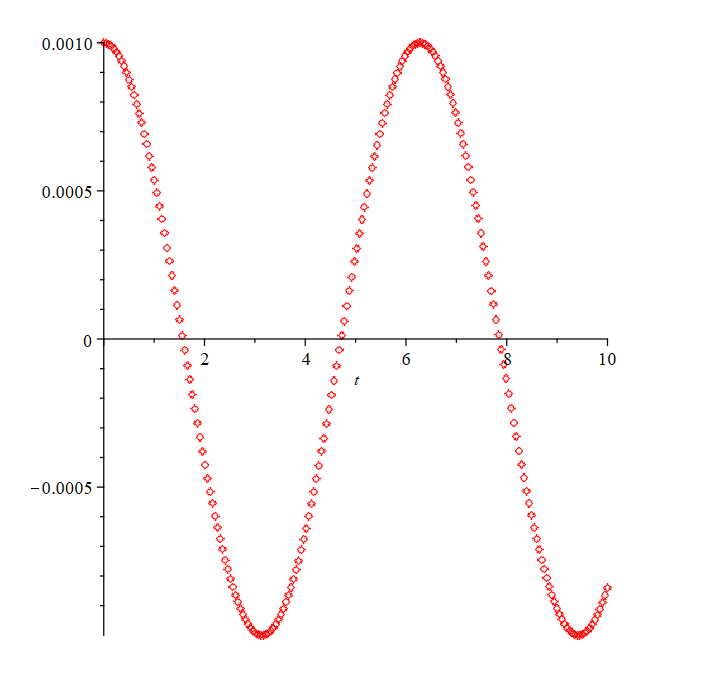
\includegraphics[width=0.5\linewidth]{n_graf1.png}}
            \end{minipage}
            \hfill
            \begin{minipage}[h]{0.5\linewidth}
            \center{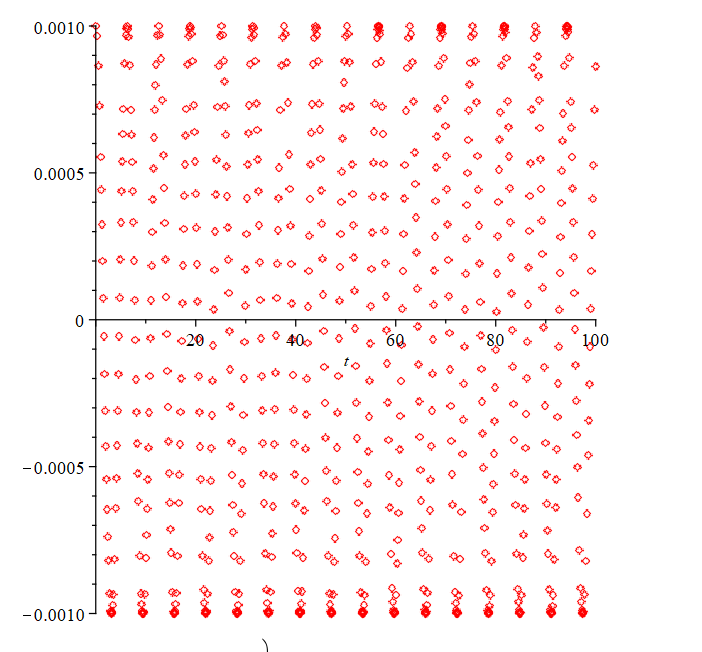
\includegraphics[width=0.5\linewidth]{n_graf2.png}}
            \end{minipage}
            \caption{График численного решения.}
        \end{figure}
        \\При помощи математического пакета  Maple, построим график функции $\frac{d^2}{dt^2}x(t) + \frac{x(t)^3}{\sqrt{(1 + x(t)^2)^3}} + x(t) = 0$
        в тех же промежутках:
        \begin{figure}[!h]
            \begin{minipage}[h]{0.5\linewidth}
            \center{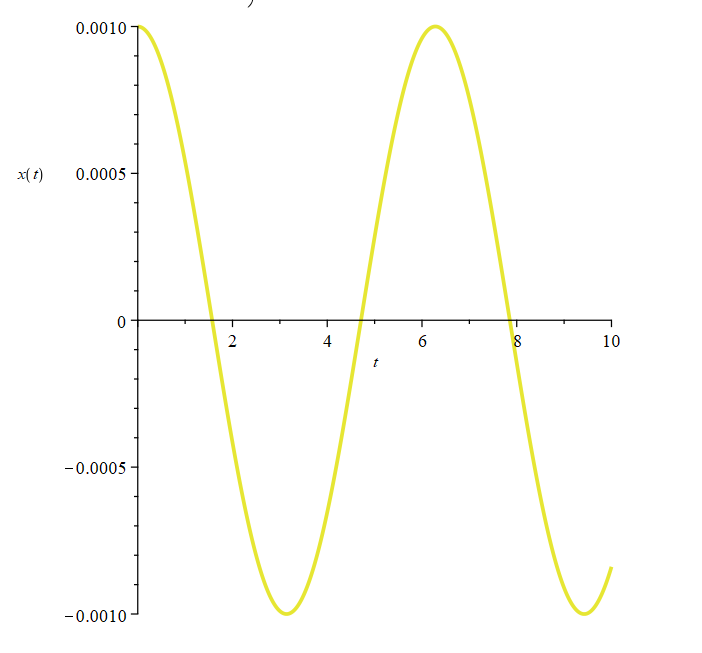
\includegraphics[width=0.5\linewidth]{e_graf1.png} }
            \end{minipage}
            \hfill
            \begin{minipage}[h]{0.5\linewidth}
            \center{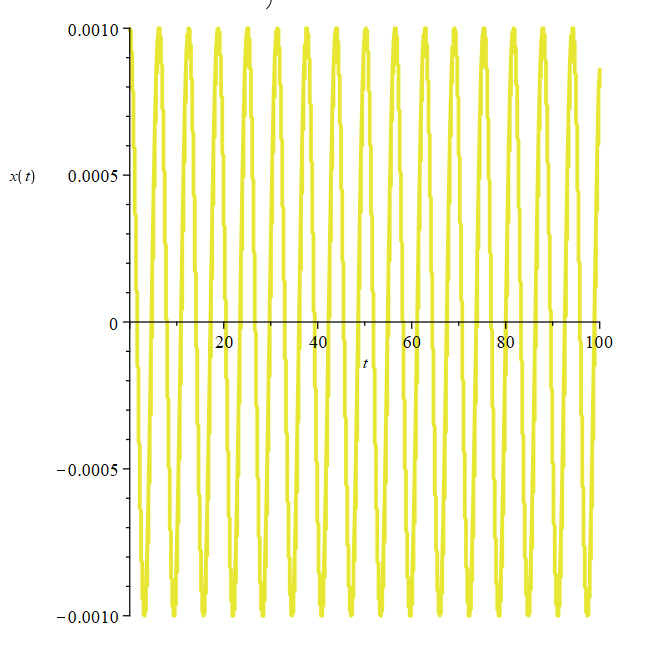
\includegraphics[width=0.5\linewidth]{e_graf2.png} }
            \end{minipage}
            \caption{График точного решения.}
        \end{figure}
        \\Наложим полученые графики друг на друга, для визуальной оценки погрешности:
        \begin{figure}[!h]
            \begin{minipage}[h]{0.5\linewidth}
            \center{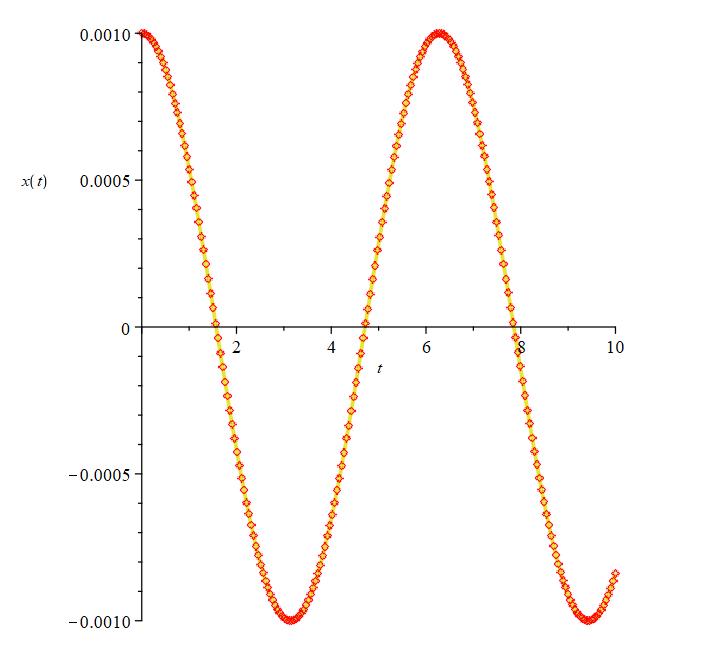
\includegraphics[width=0.5\linewidth]{en_graf1.png} }
            \end{minipage}
            \hfill
            \begin{minipage}[h]{0.5\linewidth}
            \center{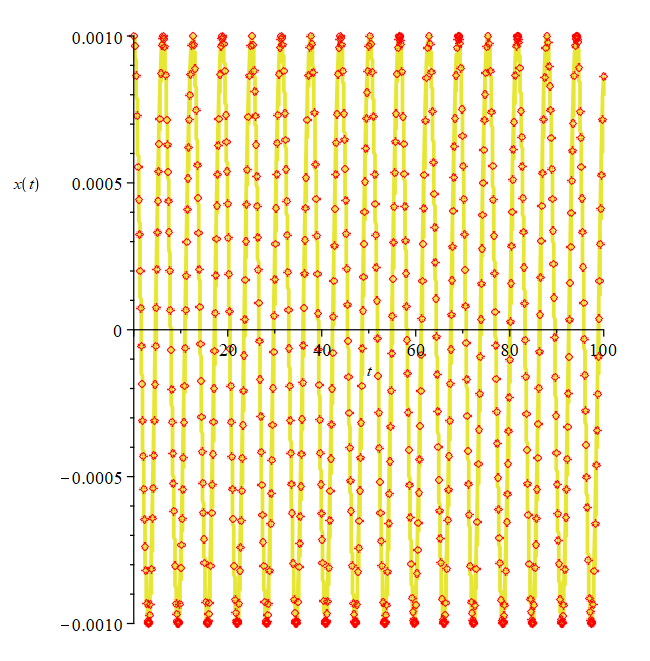
\includegraphics[width=0.5\linewidth]{en_graf2.png} }
            \end{minipage}
            \caption{Совмещенный графики.}
        \end{figure}
    \end{itemize}

\end{document}